\chapter{Исследовательский раздел}

В данном разделе описываются технические характеристики устройства. Исследуется зависимость качества изображения от коэффициента масштабирования. Также проводится сравнение методов. 

\section{Технические характеристики}

Устройство, на котором проводилось исследование, имеет следующие характеристики:

\begin{itemize}[label=---]
    \item Операционная система --- MacOS Tahoe 26.3;
    \item Процессор --- Apple silicon M5;
    \item ОЗУ --- 16 ГБ. 
\end{itemize}

\section{Сравнение методов}

На рисунках~\ref{fig:res:cmp_psnr}~---~\ref{fig:res:cmp_ssim} представлено метрическое сравнение методов. Метрическое сравнение проводилось на тестовом наборе Urban100. 

\begin{figure}[H]
    \centering
    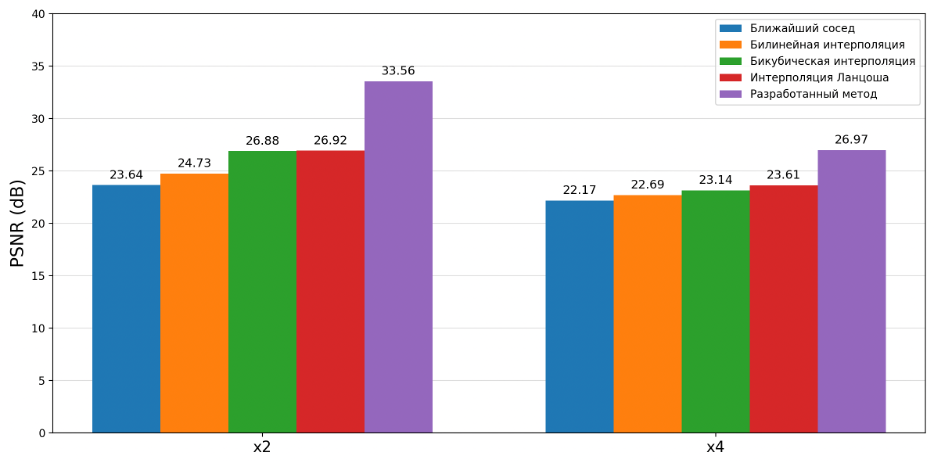
\includegraphics[width=0.9\linewidth]{images/research/cmp_psnr.png}
    \caption{Сравнение методов по PSNR}
    \label{fig:res:cmp_psnr}
\end{figure}

\begin{figure}[H]
    \centering
    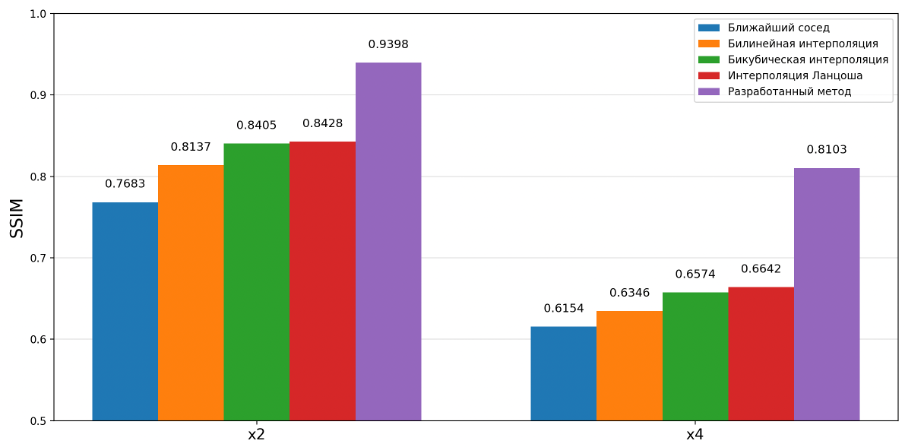
\includegraphics[width=0.9\linewidth]{images/research/cmp_ssim.png}
    \caption{Сравнение методов по SSIM}
    \label{fig:res:cmp_ssim}
\end{figure}

Визуальное сравнение методов представлено на рисунках~\ref{fig:res:vis_cmp1}~---~\ref{fig:res:vis_cmp4}. 

\begin{figure}[H]
    \centering
    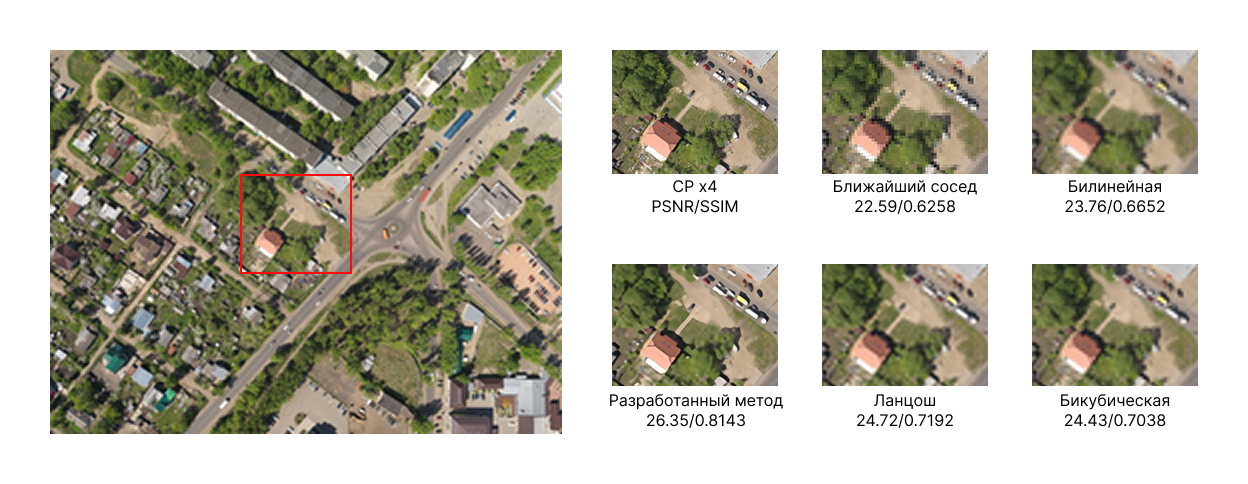
\includegraphics[width=1\linewidth]{images/research/vis_cmp_city.png}
    \caption{Визуальное сравнение методов на аэрофотоснимке города}
    \label{fig:res:vis_cmp1}
\end{figure}

\begin{figure}[H]
    \centering
    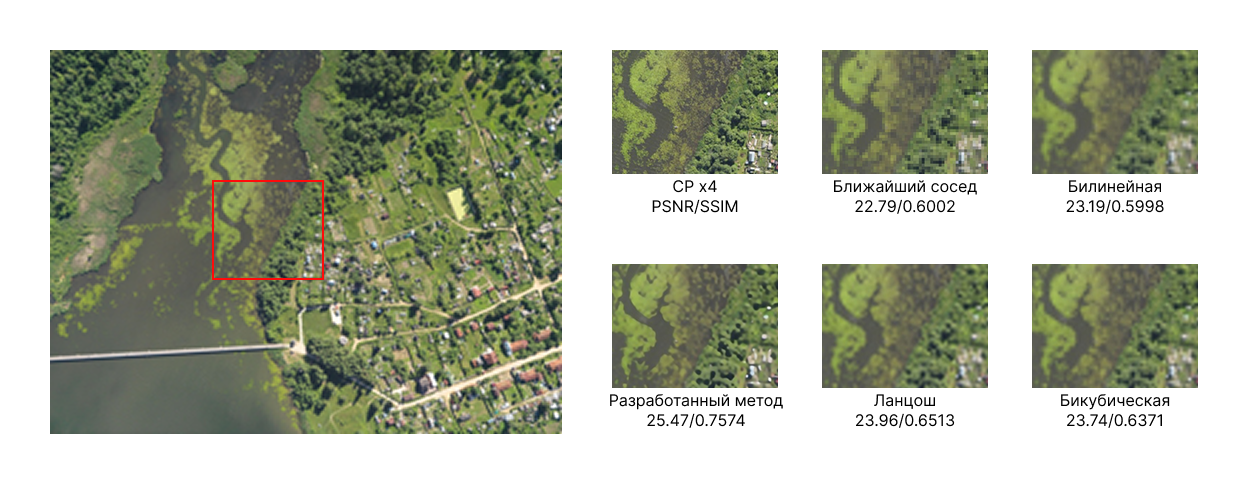
\includegraphics[width=1\linewidth]{images/research/vis_cmp_water.png}
    \caption{Визуальное сравнение методов на аэрофотоснимке воды}
    \label{fig:res:vis_cmp2}
\end{figure}

\begin{figure}[H]
    \centering
    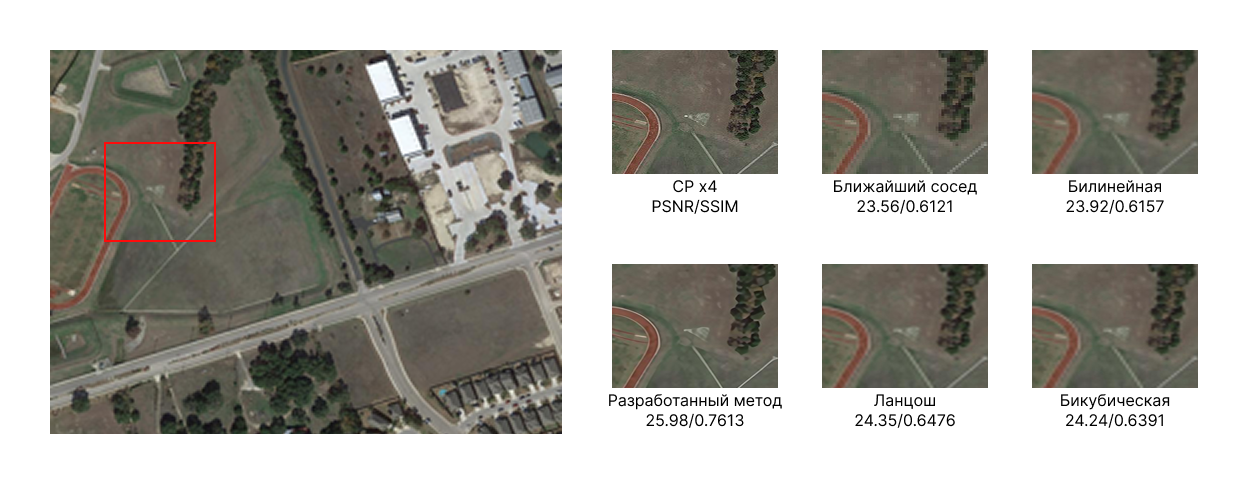
\includegraphics[width=1\linewidth]{images/research/vis_cmp_field.png}
    \caption{Визуальное сравнение методов на аэрофотоснимке поля с деревьями}
    \label{fig:res:vis_cmp3}
\end{figure}

\begin{figure}[H]
    \centering
    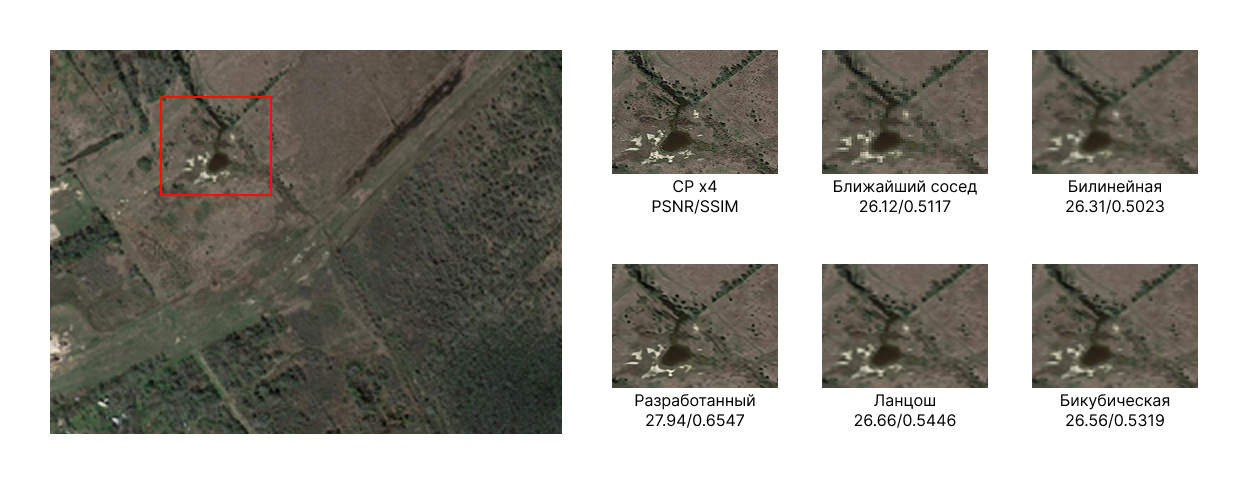
\includegraphics[width=1\linewidth]{images/research/vis_cmp_hole.png}
    \caption{Визуальное сравнение методов на аэрофотоснимке поля с водоемом}
    \label{fig:res:vis_cmp4}
\end{figure}

Сравнение проводилось с интерполяционными методами, исходя из того что они, также как и разработанный метод, поддерживают масштабирование изображений с дробными коэффициентами

Разработанный метод метрически превосходит рассматриваемые интерполяционные методы. При визуальном сравнении также заметно, что предложенный метод выделяет объекты четче, меньше размывает границы и лучше восстанавливает детали, создавая минимальное количество артефактов.

\section{Зависимость качества изображения от масштабирования}

Было проведено исследование зависимости качества изображения от коэффициента масштабирования. Исследование проводилось на тестовом наборе Urban100. Качество изображения измерялось метриками PSNR и SSIM. графики зависимостей представлены на рисунках~\ref{fig:res:res_psnr}~---~\ref{fig:res:res_ssim}.

\begin{figure}[H]
    \centering
    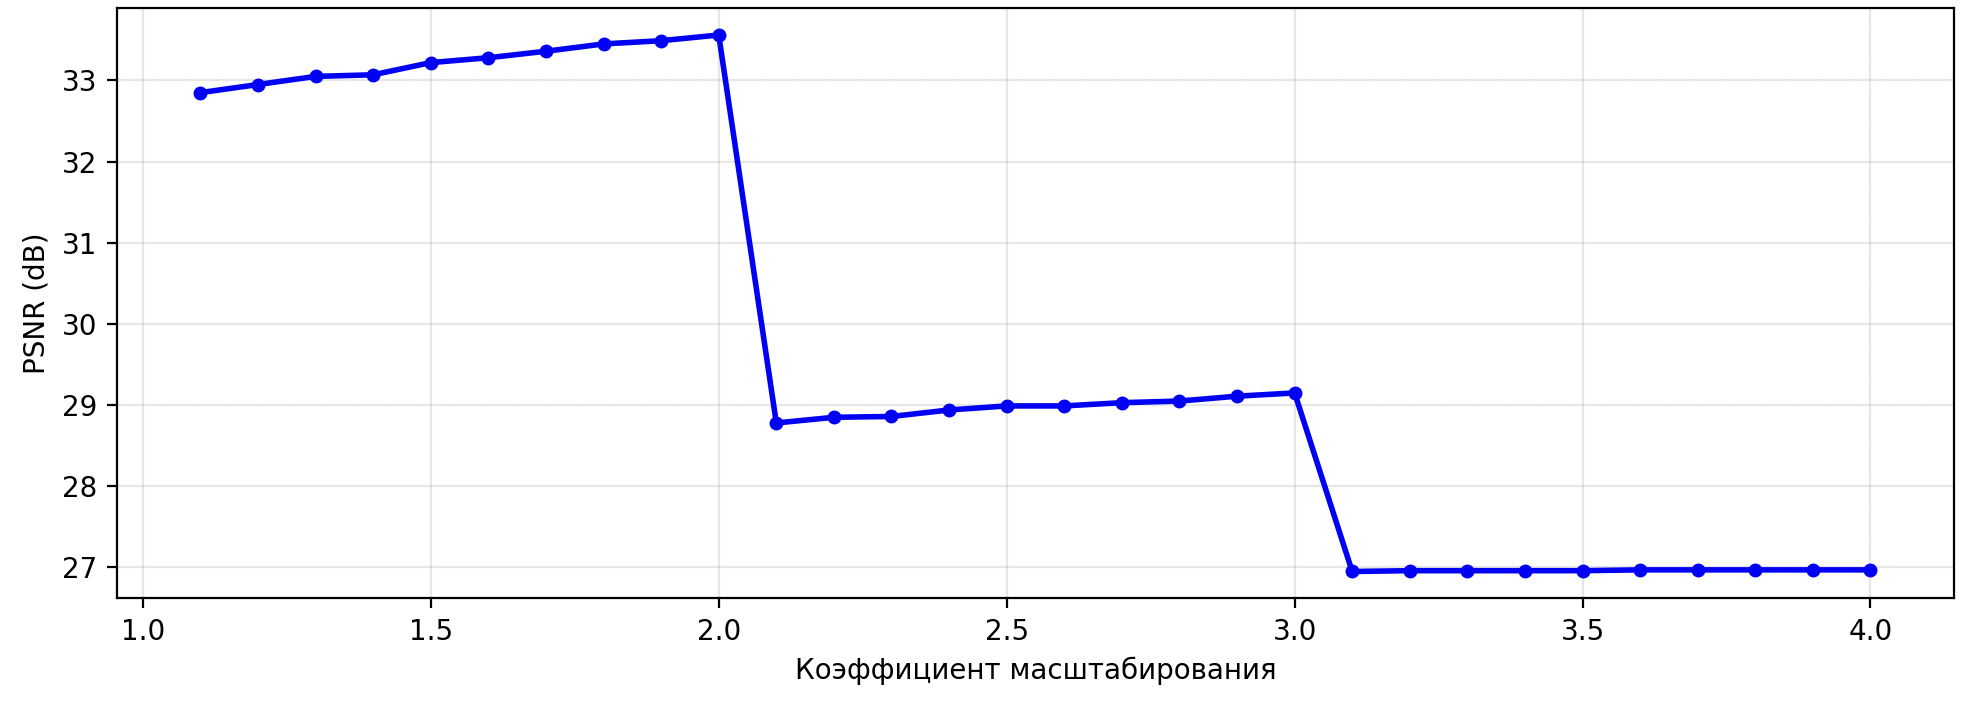
\includegraphics[width=1\linewidth]{images/research/res_psnr.png}
    \caption{Зависимость PSNR от коэффициента масштабирования}
    \label{fig:res:res_psnr}
\end{figure}

\begin{figure}[H]
    \centering
    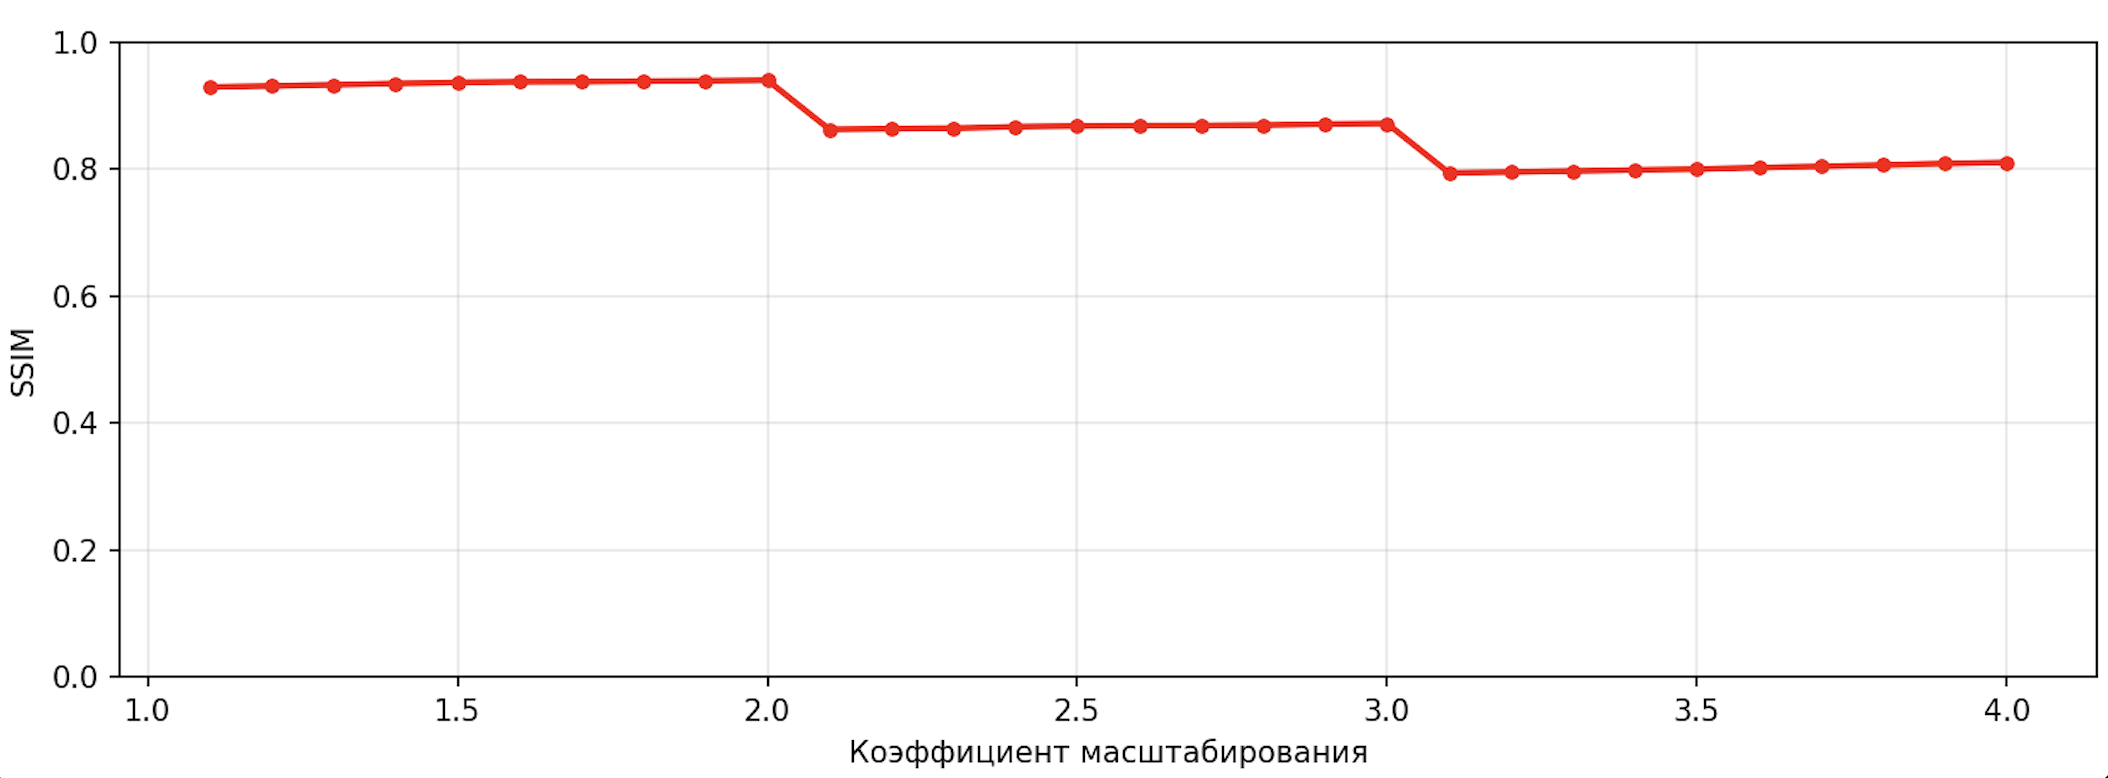
\includegraphics[width=1\linewidth]{images/research/res_ssim.png}
    \caption{Зависимость SSIM от коэффициента масштабирования}
    \label{fig:res:res_ssim}
\end{figure}

Графики зависимости метрик PSNR и SSIM демонстрируют ступенчатую зависимость качества изображения от коэффициента масштабирования. Ступенчатость возникает в момент, когда коэффициент масштабирования становится больше 2, и больше 3. В эти моменты происходит переключения между различными нейронными сетями, обученными на соответствующие коэффициенты. В промежутках где не происходит смена нейронной сети зависимость стремится к линейно-возрастающей, из чего можно сделать вывод что качество изображения при уменьшении исходного интерполяцией падает, но превосходит качество полученное повышением разрешения только интерполяционными методами. 

\section*{Вывод}
\addcontentsline{toc}{section}{Вывод}

В данном разделе описаны технические характеристики устройства. Была исследована зависимость качества изображения от коэффициента масштабирования. Исследование показало ступенчатую зависимость при смене нейронной сети и линейно-возрастающую в промежутке работы одной нейронный сети. Проведено сравнение методов, которое показало что разработанный метод превосходит рассмотренные интерполяционные методы. 